\chapter{Studies of inconsistency indexes for incomplete matrices}
\label{sec:studiesOfInconsistencyIndexesForIncompleteMatrices}

The presented inconsistency indexes have been tested utilizing the Monte Carlo method. Their aim was to select those indexes which will give reliable results for incomplete matrices. Therefore, it was decided that the measure of the indexes' quality would be a \textit{relative error} (expressed as a percentage), which took into account the value of the index for a full, inconsistent matrix and the value of the index for the same matrix after partial decomposition. To be sure that the results were fair, all indexes were tested on the same set of matrices. The different sizes of the matrices, the levels of incompleteness and the levels of inconsistency were taken into account. Then, in order to compare the indexes easily and to select the best ones, the results were averaged using the arithmetic mean. While building the algorithm to solve the problem (Kazibudzki, 2017) was used.


\section{Algorithm}
\subsection{Steps of the algorithm}
\textbf{The algorithm of test of inconsistency indexes:}
\begin{enumerate}
\item Randomly generate a vector $w=[w_{1},...,w_{n}]$ and a consistent \textit{PCM matrix} associated with it $PCM=\left(m_{ij}\right)$, where $m_{ij}=\frac{w_{i}}{w_{j}}$.
\item Disrupt the matrix by multiplying its elements (excluding the diagonal) by the value of $d$, randomly selected from the range $\left(\frac{1}{x},x\right)$.
\item Replace values $m_{ij}$, where $i<j$ by values $m_{ji}$.

\item Calculate values of index with all methods for the created matrix.

\item Remove some values from the matrix by removing some of values. The level of incompleteness should be $g$\%.

\item Calculate the values of inconsistencies by all methods for the decomposed matrix.

\item Calculate the relative error for each index.

\item Repeat steps 1 to 10 $X_{1}$ times.

\item Calculate the average relative error for each inconsistency index for the \textit{PCM matrix}.

\item Repeat steps 1 to 10 $X_{2}$ times.

\item Calculate the average relative error for each index by averaging the values obtained in step 9.

\end{enumerate}


\subsection{Details of algorithm}
The above algorithm was carried out for values $X_{1}=100$, $X_{2}=100$. Tests were started for values d in the range $\left(1.1,1.2,...,4\right)$ and then the results were averaged. It means that the average relative error of one index was calculated on the basis of 4000 matrices, each of which decomposed randomly 100 times. It gave together 400000 tests how good the index was. 
\\

In addition, tests were carried out for various sizes of matrices.\\
\textbf{The results are divided into two parts:}
\begin{enumerate}
  \item A constant degree of incompleteness, different size of the matrix.
  \item Different degrees of incompleteness, constant size of the matrix.
\end{enumerate}

The aim of such a division is to pay attention to how the inconsistency indexes behave when the size of the matrix and the degree of incompleteness are changing. The results of the research are presented below.


\section{Implementation}

\subsection{Development environment}
Testy współczynników zostały napisane w języku R, który idealnie nadaje się do obliczeń numerycznych. Posiada on szereg funkcji, które wspierą działania na macierzach i wektorach. W~czasie implementacji wykorzystano integrated development environment (IDE) o nazwie RStudio. Narzędzie to pozwala na tworzenie własny pakietów, które zawierają nie tylko właściwy, ale również dokumentację, czy informacje o licencji i autorze. Utworzono pakiet o nazwie \textit{indexesForIncomplete}. Najważniejszą częścią pakietu jest plik indexes.R, który wykonuje obliczenia konieczne do zbadania współczynników. RStudio wspomaga pracę programisty poprzez kolorowanie składni, wbudowaną konsole, łatwe przeszukiwanie funkcji i dokumentacji oraz wiele innych. Program dostępny jest na wszystkie popularne systemy operacyjne. Aby korzystać z RStudio należy wcześniej zainstalować język~R.
% https://pbiecek.gitbooks.io/przewodnik/content/Programowanie/podstawy/jak_zainstalowac_R.html
% https://cran.r-project.org/
% https://www.rstudio.com/products/RStudio/
\begin{figure}[ht]
\centerline{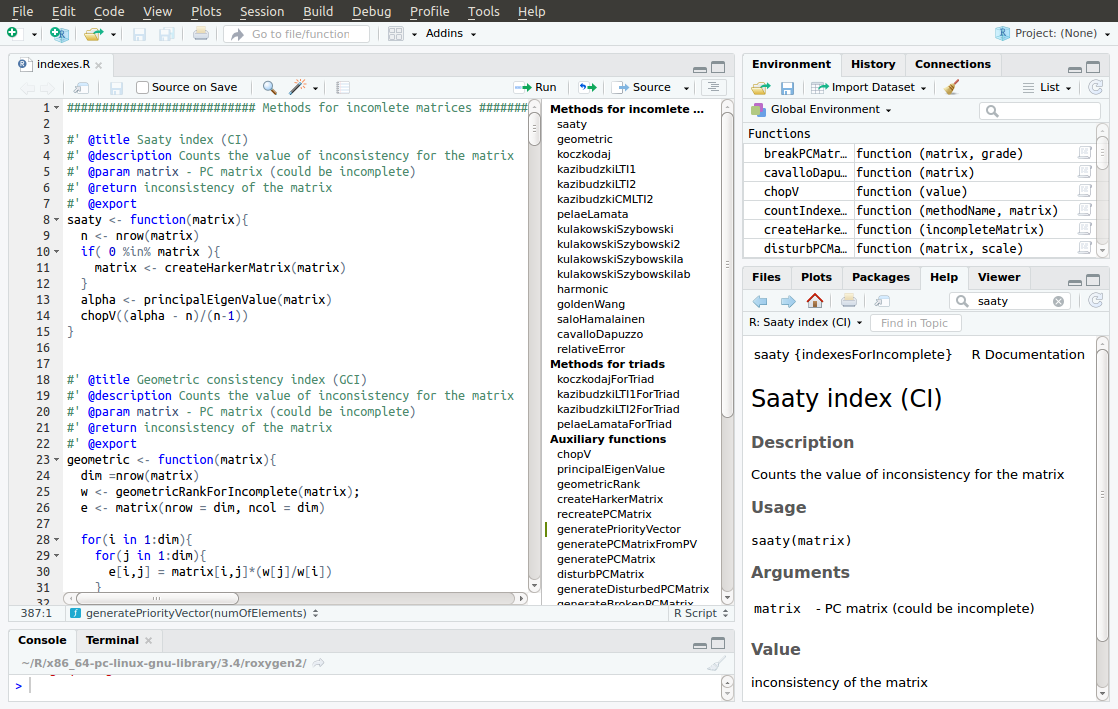
\includegraphics[width=\textwidth]{images/rstudio.png}}
\caption{Program \textit{RStudio}}
\label{fig:rstudio}
\end{figure}


\subsection{Implementation of tests inconsistency indexes}
Implementacja testów współczynników niespójnności to składała się z dwóch kroków:
\begin{enumerate}
  \item Implementacja funkcji, które obliczają współczynniki niespójności dla zadanej macierzy (pełnej lub niepełnej).
  \item Implementacja testów, które zbadają współczynniki dla różnych macierzy i zbiorą wyniki tych testów.
\end{enumerate}

\subsubsection{Implementacja współczynników niespójności}
Utworzono 16 funkcji, które obliczają współczynnik niespójnności metodami, które zostały opisane powyżej. Funkcje zostały napisane w taki sposób, że potrafią poradzić sobie zarówno z macierzami pełnymi, jak również niepełnymi. Nie uwzględeniono błędnych macierzy, a więc takich, które niespełniają założeń symetrycznej, spójnej PC macierzy. Każda funkcja posiada tylko jeden argument, którym jest PC macierz. Wyjątkiem są dwie funkcje implementujące współczynniki Koczkodaja i Szybowskiego, które dodatkowo przyjmują parametry $\alpha, \beta$. Wynikiem działania  funkcji jest wartość współczynnika niespójności.
Każda funkcja została uzupełniona o komentarze, które informują m.in o nazwie współczynnika, któremu funkcja odpowiada, parametrach i zwracanej wartości. Pozwala to z łatwością czytać kod i wprowadzać do niego poprawki.
Kilka przykładów funkcji zostało zaprezentowanych poniżej.

\begin{figure}[ht]
\centerline{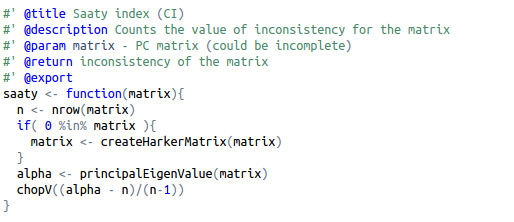
\includegraphics[scale=0.75]{images/kod1.png}}
\caption{Implemetnacja współczynnika \textit{Saaty'ego}}
\label{fig:rstudio}
\end{figure}

\begin{figure}[ht]
\centerline{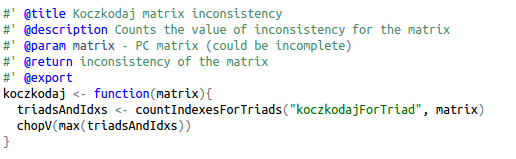
\includegraphics[scale=0.75]{images/kod2.png}}
\caption{Implemetnacja współczynnika \textit{Koczkodaja}}
\label{fig:rstudio}
\end{figure}

\begin{figure}[ht]
\centerline{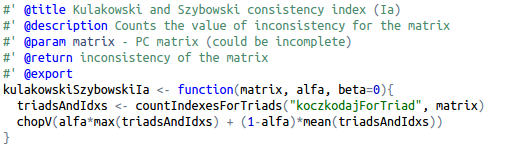
\includegraphics[scale=0.75]{images/kod3.png}}
\caption{Implemetnacja współczynnika \textit{Kulakowskiego i Szybowskiego}}
\label{fig:rstudio}
\end{figure}

\begin{figure}[ht]
\centerline{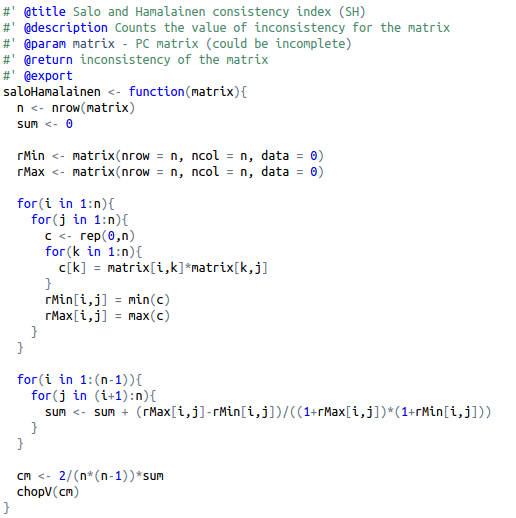
\includegraphics[scale=0.75]{images/kod4.png}}
\caption{Implemetnacja współczynnika \textit{Salo i Hamalainen}}
\label{fig:rstudio}
\end{figure}
Warto zwrócić uwagę na funkcję, która zostaje wywołana wewnątrz funkcji przeznaczonych dla współczynników opartych na triadach. Generuje traidy z macierzy, a następnie oblicza niespójność dla każdej z nich. Sposób obliczenia niespójności dla triady jest jednak zależny od pierwszego argumentu funkcji, gdzie podawana jest nazwa funkcji, potrafiącej obliczyć niespójność triady konkretną metodą.

\begin{figure}[ht]
\centerline{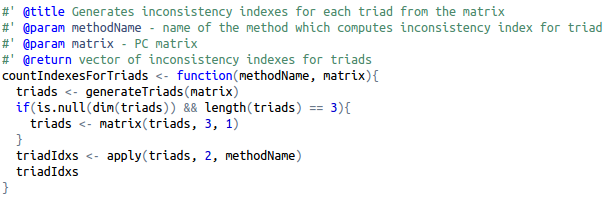
\includegraphics[scale=0.75]{images/kod5.png}}
\caption{Implemetnacja metody \textit{countIndexesForTriads}, która oblicza wartość niespójności dla każdej triady zadanej macierzy}
\label{fig:rstudio}
\end{figure}


\subsubsection{Implementacja testów}
W drugim kroku otworzono funkcje, które pozwalają obliczyć jakość współczynników dla macierzy niepełnych. W tym procesie ważną rolę odgrywają funkcje generujące określone macierze. PC macierze generowane są w zależości od wymiaru, wielkości niespójności i stopnia niekompletności.

\begin{figure}[!ht]
\centerline{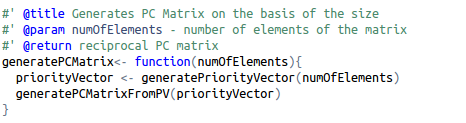
\includegraphics[scale=0.75]{images/kod11.png}}
\caption{Implemetnacja funkcji \textit{generatePCMatrix}, która generuje PC macierz w zależności od rozmiaru}
\label{fig:rstudio}
\end{figure}

\begin{figure}[!ht]
\centerline{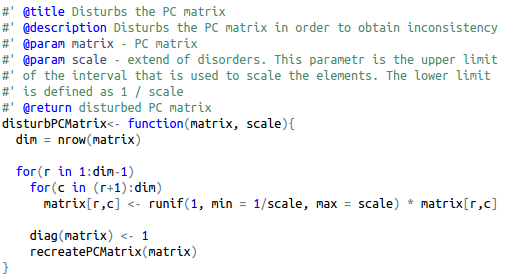
\includegraphics[scale=0.75]{images/kod12.png}}
\caption{Implemetnacja funkcji \textit{disturbPCMatrix}, która zaburza macierz powodując niespójność w zależności od zadanej skali }
\label{fig:rstudio}
\end{figure}

\begin{figure}[!ht]
\centerline{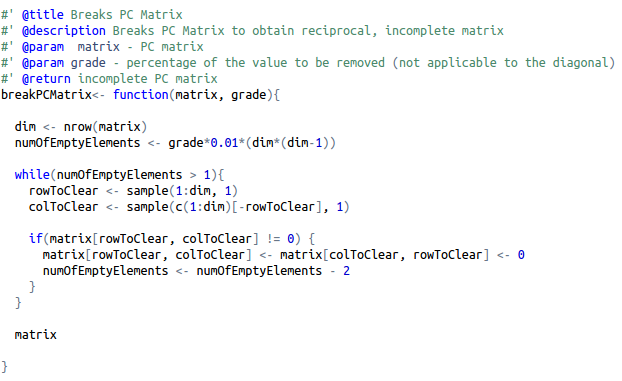
\includegraphics[scale=0.73]{images/kod13.png}}
\caption{Implemetnacja funkcji \textit{breakPCMatrix}, która dekompletuje macierz powodując niekompletność w zależności od zadanej skali}
\label{fig:rstudio}
\end{figure}

Ostatnia część funkcji dotyczy testowania jak duży błąd względny występuje dla współczynników niespójności po ich zdekompletowaniu. Najpierw utworzono funkcję, która testuje jeden współczynnik. Bierze pod uwagę rozmiar, wielkość niespójności, poziom niekompletności i ilość prób, które są przeprowadzane dla danej macierzy.

\begin{figure}[!ht]
\centerline{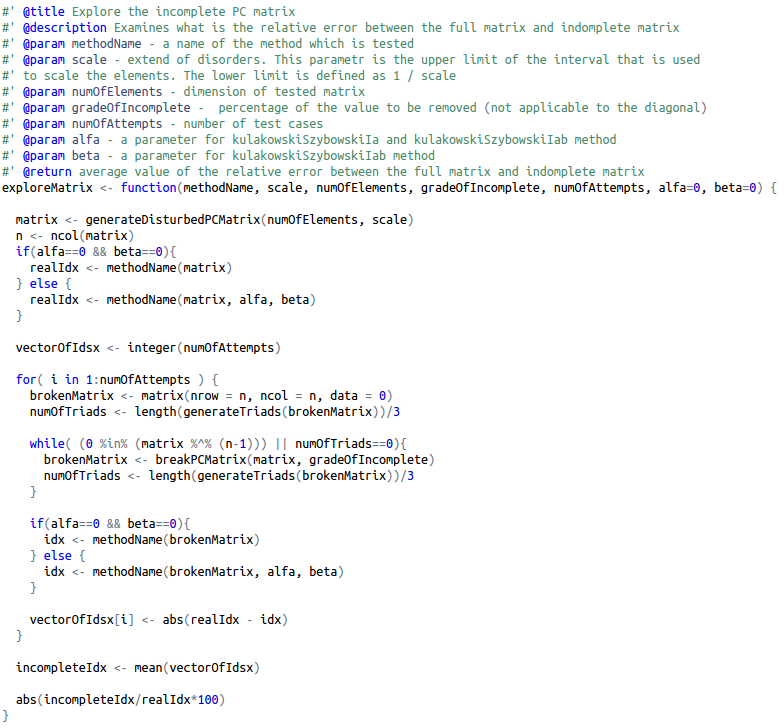
\includegraphics[scale=0.58]{images/kod21.png}}
\caption{Implemetnacja funkcji \textit{exploreMatrix}, która testuje wybrany współczynik niespójności}
\label{fig:rstudio}
\end{figure}

Następnie zostały utworzone funkcje, które przeprowadzają testy dla wszystkich współczynników, opierając się na tych samych macierzach. Dzięki temu zbiór macierzy, na których operuję współczynniki są jest wspólny, zatem rezultaty są wiarygodne, a każdy współczynnik jest traktowany w ten sam sposób.

\begin{figure}[!ht]
\centerline{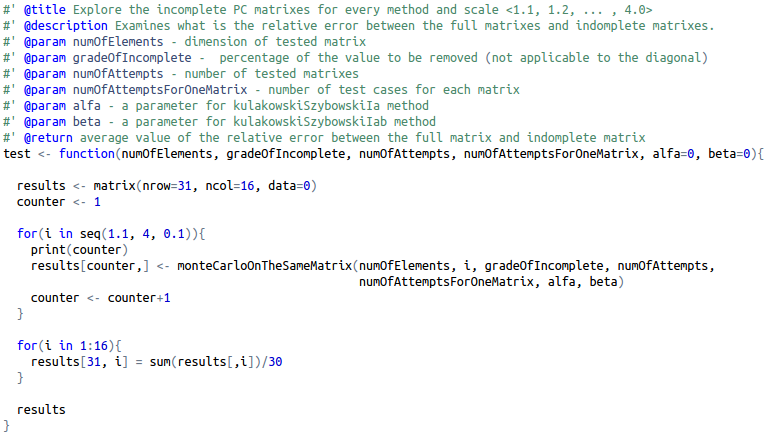
\includegraphics[scale=0.58]{images/kod22.png}}
\caption{Implemetnacja funkcji \textit{test}, która testuje wszystkie współczynniki, uwzględniając zadany rozmiar macierzy i stopień niekompletności}
\label{fig:rstudio}
\end{figure}


\subsection{Documentation}
Komentarze kodu zostały wykorzystane do wygenerowania dokumentacji. W tym celu użyto pakietu \textit{roxygen2}. Pozwoliło to na łatwe przeglądanie funkcji przyjemne zapoznanie się z nimi.
Przykładowe fragmenty dokumentacji przedstawione zostały poniżej.

\begin{figure}[!ht]
\centerline{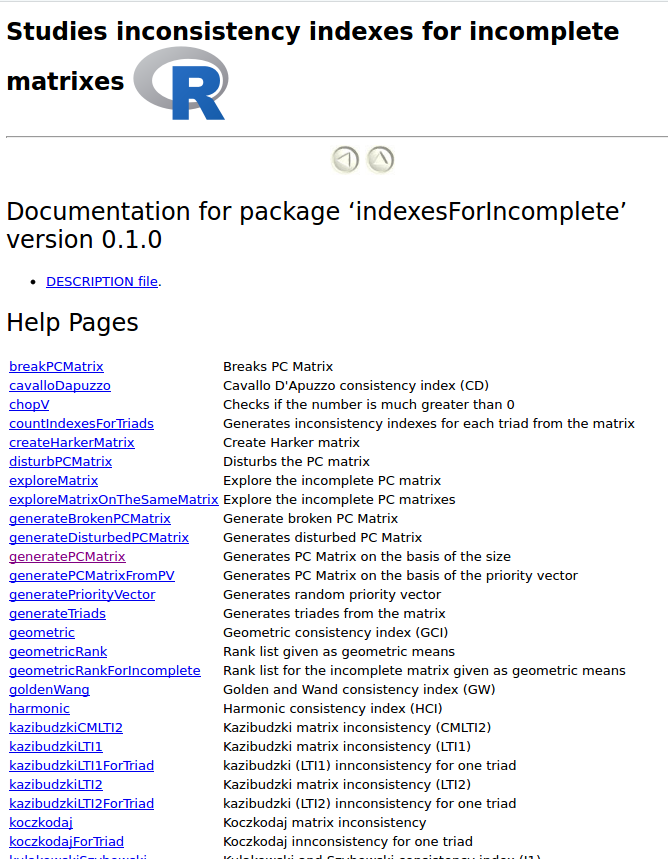
\includegraphics[scale=0.58]{images/kod31.png}}
\caption{Fragment dokumentacji: widok ogólny}
\label{fig:rstudio}
\end{figure}

\begin{figure}[!ht]
\centerline{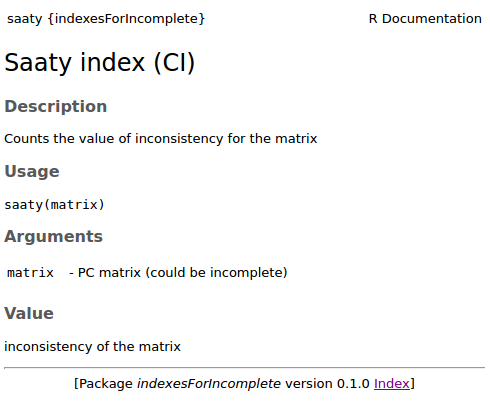
\includegraphics[scale=0.58]{images/kod32.png}}
\caption{Fragment dokumentacji: funkcja \textit{saaty}}
\label{fig:rstudio}
\end{figure}

\begin{figure}[!ht]
\centerline{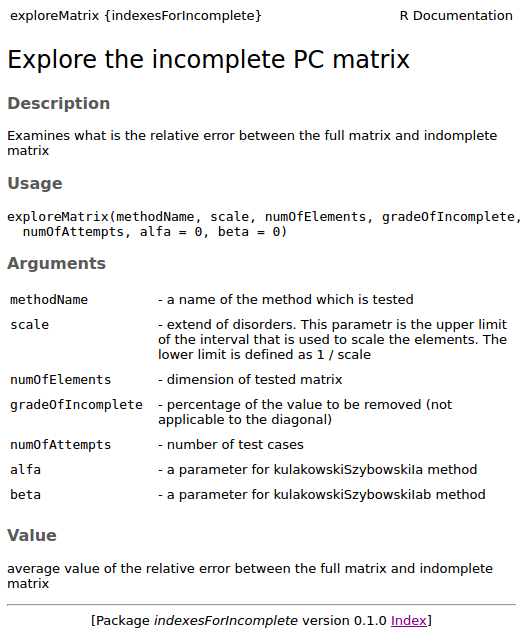
\includegraphics[scale=0.58]{images/kod33.png}}
\caption{Fragment dokumentacji: funkcja \textit{exploreMatrix}}
\label{fig:rstudio}
\end{figure}